\subsection{Robustness Analysis}\label{sec:robustness}
Each sensitivity analysis specifies its population and uncertainty model.
\subsubsection{Sensitivity to Sampling and References}\label{sec:precision}
For the first-release gap difference $-0.0556925$, 1,000 bootstrap draws resample paired tasks within domain/stratum and references within domain, retaining joint model responses. The conditional 95\% interval is $[-0.0665464,-0.0434725]$.

Leave-one-domain-out contrasts and all 56 three-of-eight means retain the favorable direction. These checks condition on observed pools and omit independent construction variance.

\paragraph{A revised target reference}
We evaluate all 417 same-domain items in BIRD's October 2026 Mini-Dev SQLite revision.\footnote{\url{https://github.com/bird-bench/mini_dev}} Question and database hashes match the publisher manifest and original snapshots; references do not overlap by domain/question/evidence identity. All SQL executes; 67 predictions truncate.

Revised-reference gap favors S2B over Template in six domains, with California/Formula 1 unresolved (Table~\ref{tab:reference-stress}); S2B-minus-Ring is $[+0.040718,+0.103446]$. The unpaired revision has more tasks rated hard by the SQL complexity measure and more nested SELECTs; domains and source TEF are unchanged.

\subsubsection{Semantic Assessment}\label{sec:semantic}
OpenAI's \texttt{gpt-6-astra} API judges question--SQL agreement \citep{zheng2023judge,liu2023geval} from question, schema and SQL with a fixed prompt and medium reasoning, blind to methods/scores. Qwen/Terra cross-check supported/incorrect/insufficient labels. Evaluator biases \citep{wang2024faireval} preclude treating these as human truth or calibrated confidence; sensitivity relaxes flagged scores at fixed denominators.

\paragraph{Generated-task audits}
An earlier stratified 400-task audit also leaves Synth unresolved under Terra's 135/137-concern scenarios. Retaining only 654 nonempty Synth roundtrip matches gives ten-release mean TEF bounds $[-1.076911,+0.283264]$; other scores are unknown at the fixed denominator.

The expanded audit fixes 100 records per method/domain, with one unavailable (Table~\ref{tab:audit-expanded}); exposed controls score 24/24 per class. The union of 1,133 audit concerns and 620 earlier SQL flags relaxes 1,433 items at the original denominators.

\begin{table}[t]\centering\small
\caption{API judgments. S/I/U: supported/incorrect/insufficient; NA/inv.: unavailable/invalid. Panels (b)/(c) compare judges on shared references and paired questions under the same Terra protocol.}
\label{tab:audit-expanded}
\begin{tabular}{lrrrr}\toprule
\multicolumn{5}{l}{\textit{(a) Astra: 800 tasks/method, 100/domain}}\\
Method & S & I & U & NA/inv.\\\midrule
Template &800&0&0&0\\
S2B &732&17&51&0\\
Ring &603&123&73&1\\
Omni &290&418&92&0\\
Synth &442&308&50&0\\\midrule
\multicolumn{5}{l}{\textit{(b) References: 160 tasks, 20/domain}}\\
Judge / parsing rule & S & I & U & NA/inv.\\\midrule
Terra &89&54&17&0\\
Qwen: strict JSON &76&9&1&74\\
Qwen: code-fence parsing &121&37&2&0\\\midrule
\multicolumn{5}{l}{\textit{(c) Terra: 160 paired tasks, 20/domain}}\\
Original S2B &141&14&5&0\\
Rewritten S2B &117&32&10&1\\\bottomrule
\end{tabular}\end{table}

Relaxing all 1,433 flags preserves S2B's TEF advantage over Template, $[-0.179682,-0.050176]$, but leaves external contrasts unresolved. Shared-source LP bounds for Ring/Omni/Synth are $[-0.293390,+0.139461]$, $[-0.840707,+0.132174]$ and $[-0.587412,+0.236106]$; joint gap bounds also cross zero. Three of 48 LP/mixed-integer gap endpoints reach time limits. Outward tolerances and earlier wider bounds remain.

\paragraph{Target-reference audits}
Accepting JSON inside code fences gives Qwen/Terra agreement on 107/160 references (Table~\ref{tab:audit-expanded}(b)); independently generated SQL sometimes contradicts the labels. The 105-item strict union treats format failures and non-supported judgments as risks, not established errors.

\begin{table*}[t]\centering\small
\caption{S2B-minus-Template gap sensitivities on the first Verified release. Each risk set retains its denominator and unflagged scores; ranges bound unknown scores.}
\label{tab:reference-stress}
\begin{tabular}{llrr}\toprule
Generated-task concerns & Reference condition & Reference count & Direct gap difference\\\midrule
None added & Original reference &906&$-0.055693$\\
1,433 union flags & Original reference &906&$[-0.077344,-0.026784]$\\
None added & 71 Terra reference concerns &906&$[-0.098374,-0.010170]$\\
137 original audit flags & 105 strict Terra/Qwen concerns &906&$[-0.114491,+0.013951]$\\
137 original audit flags & 79 code-fence sensitivity concerns &906&$[-0.105686,-0.002284]$\\
None added & Revised BIRD reference &417&$[-0.076995,-0.024912]$\\
1,433 union flags & Revised BIRD reference &417&$[-0.105428,+0.000213]$\\\bottomrule
\end{tabular}\end{table*}

The 71-reference scenario favors S2B in all ten releases. Combining strict cross-check or revised references with generated risks leaves the first release unresolved (Table~\ref{tab:reference-stress}). Reference-only changes leave TEF unchanged.

\subsubsection{Sensitivity to Question Rewriting}\label{sec:risk-sources}
Figure~\ref{fig:risk-sources} separates construction (43 rewritten, seven original S2B, 23 Ring) and reference risks (71 Terra or 105 strict Terra/Qwen). Each flag relaxes all ten scores, fixing others and sharing source/reference variables. ``Both'' combines flags, excluding the separate 1,433-item union.

\begin{figure*}[t]
\centering
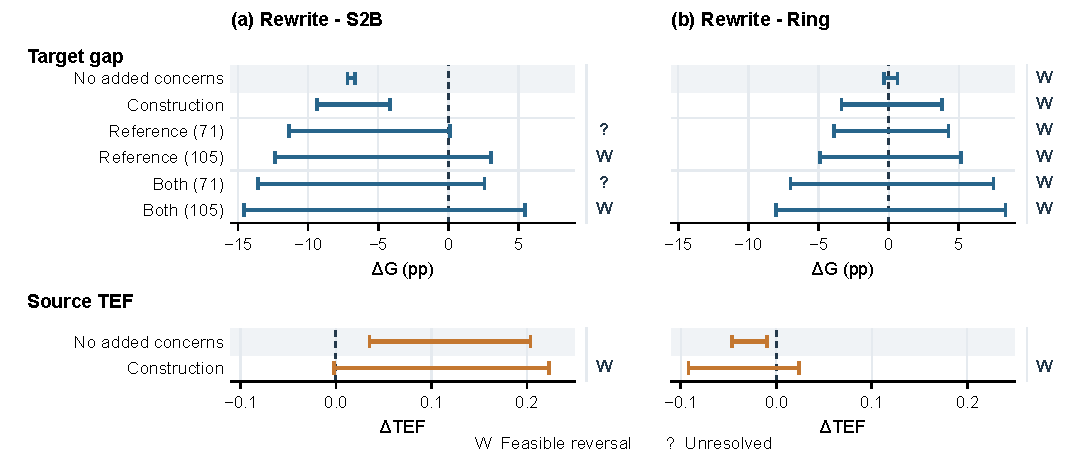
\includegraphics[width=\textwidth]{figures/current/Fig5.pdf}
\caption{Sensitivity of rewriting with fixed SQL using earlier audit flags. Target gap is above source TEF. W: a feasible score assignment reverses the comparison; ?: search unresolved; blank: not searched.}
\label{fig:risk-sources}
\end{figure*}

Construction flags preserve the rewrite's gap advantage but leave both TEF contrasts unresolved. Either reference-risk set makes gap direction unresolved without changing TEF.

Positive differences are feasible in 14/16 Verified cases whose bounds cross zero; this establishes neither semantic errors nor reversal probabilities.

Terra reviews 160 paired originals under the same protocol (Table~\ref{tab:audit-expanded}(c)). Combined flags cover 24 original, 43 rewritten, 23 Ring and 71 reference items. Verified rewrite-minus-original gap $[-0.142130,+0.032135]$ and TEF $[-0.008539,+0.235566]$ are both unresolved.

\subsubsection{Metric Weights and Model Coverage}\label{sec:sensitivity}
Accuracy and the correct-count CDF favor S2B against all comparators; disagreement favors it over Template, is adverse to Ring ($[+0.012123,+0.066481]$), and unresolved for Omni/Synth. Equal component weights and pooled-task averaging leave S2B-minus-Synth unresolved: $[-0.400081,+0.034253]$ and $[-0.430144,+0.025669]$. Template/Ring/Omni directions persist.

Figure~\ref{fig:weights} varies nonnegative accuracy/CDF/disagreement weights summing to 2.5 on the first Verified release without semantic flags. Colors classify regions as favorable, adverse or unresolved using conservative bounds, without assigning probabilities.

\begin{figure*}[t]
\centering
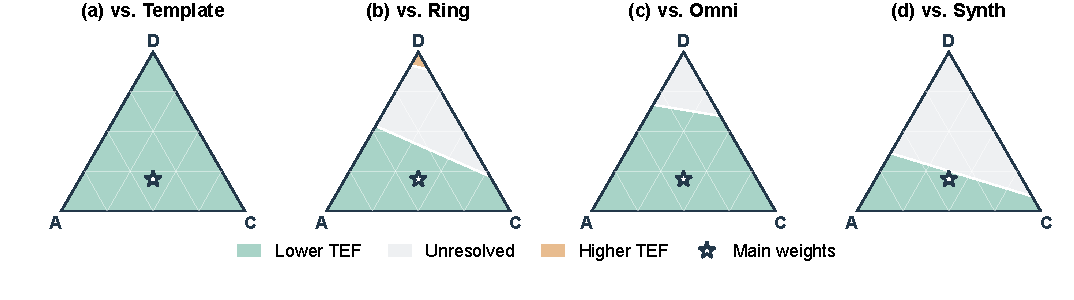
\includegraphics[width=\textwidth]{figures/current/Fig6.pdf}
\caption{Post-hoc TEF weight sensitivity. A: accuracy; C: correct-count CDF; D: disagreement. Star: original weights $(1,1,0.5)$.}
\label{fig:weights}
\end{figure*}

S2B beats Template throughout the weight region. Emphasizing disagreement can favor Ring and leaves Omni/Synth unresolved.

Removing Qwen retains favorable Verified TEF contrasts after recomputing normalizers; external adaptations still have lower gap (Table~\ref{tab:panel-coverage}). Summary/DDL source prompts both favor S2B over Template, with unresolved direct difference.

Broader coverage retains the Template--S2B gap advantage (Table~\ref{tab:panel-coverage}). Adding Qwen3.6-27B, Qwen3.8-27B, Gemma 3 4B and OLMo 2 7B tests model coverage, without resolving exclusion bias, transfer or training overlap.

\begin{table*}[t]\centering\small
\caption{Eight-database gap sensitivity: positive $I_G=G(\mathrm{Template})-G(\mathrm{S2B})$ favors S2B. Conditional confidence intervals (CIs) resample within domains; bounds describe unknown scores.}
\label{tab:panel-coverage}
\begin{tabular}{lrrrl}\toprule
Setting & Pairs & References & Gap improvement $I_G$ & Interpretation\\\midrule
Non-Qwen panel &2,000&906&$0.026560$&Ten-release mean\\
Broader reference coverage &3,778&982&$0.053302\ [0.041870,0.063207]$&Conditional 95\% CI\\
Equal-skeleton weighting &3,778&982&$0.046936\ [0.034298,0.057670]$&Conditional 95\% CI\\
Full available pool &3,835&1,118&$[0.009303,0.090704]$&Unknown-score bound\\\midrule
Fourteen models: strict &2,000&906&$[0.002662,0.059226]$&Unknown-score bound\\
Fourteen models: database checks &2,000&906&$[0.025795,0.032495]$&Unknown-score bound\\
Fourteen models: strict &3,778&906&$[0.002188,0.059640]$&Unknown-score bound\\
Fourteen models: database checks &3,778&906&$[0.025787,0.032648]$&Unknown-score bound\\\bottomrule
\end{tabular}

\smallskip\parbox{\textwidth}{\footnotesize The full-pool setting uses 8,788 prompts/model. The 2,000-pair fourteen-model rows average bound endpoints over ten overlapping releases. Fourteen-model concordances/inversions are 567/136 for 2,000 pairs and 533/168 for 3,778 pairs, each out of 728 dependent model pairs.}
\end{table*}

LIMIT counts are 1,739/2,000 for Template/S2B, 1,753 Ring, 424 Omni and 872 Synth, versus 62/906 references. Only 108/240 method--domain--structure cells (10/40 LIMIT cells) have ten tasks in both populations, preventing complete matched analysis. A pilot table-name repair does not apply to the retained failed outputs.

\subsection{Generalization Experiments}\label{sec:external}
\begin{table*}[t]\centering\small
\caption{External-pilot differences (S2B minus comparator); negative favors S2B. TACO: 750 tasks/method, 595 references, database and reference checks. BEAVER: 472 tasks/method, all 194 references. Scoring layers and schemas are separated. Each pilot uses matching source context, pooled TEF and gap averaged across domains.}
\label{tab:external-pilot}
\begin{tabular}{llrr}\toprule
Setting & Comparator & $\Delta\mathrm{TEF}$ & $\Delta G$\\\midrule
TACO: retrieved schema & Template & $[-0.006024,+0.016398]$ & $[-0.030517,+0.044555]$\\
TACO: retrieved schema & Ring & $[+0.133673,+0.280760]$ & $[+0.148866,+0.277121]$\\\midrule
BEAVER: retrieved, Base & Template & $[-0.146373,-0.033660]$ & $[-0.081035,+0.060364]$\\
BEAVER: retrieved, Base & Ring & $[-0.242054,-0.013075]$ & $[-0.056789,+0.099330]$\\
BEAVER: oracle schema, Base & Template & $[-0.142702,-0.028519]$ & $[-0.083884,+0.049262]$\\
BEAVER: oracle schema, Base & Ring & $[-0.130602,+0.168975]$ & $[-0.051570,+0.064633]$\\\midrule
BEAVER: retrieved, Verified & Template & $[-0.146163,-0.037765]$ & $[-0.081035,+0.060364]$\\
BEAVER: retrieved, Verified & Ring & $[-0.235815,-0.016203]$ & $[-0.056789,+0.099330]$\\\bottomrule
\end{tabular}\end{table*}

TACO OpenData \citep{deng2026taco} supplies two related Beijing databases and Connecticut, with potentially synthetic references. Admission and initial sampling differ from the main study. With 16 retrieved objects, contrasts are unresolved against Template and adverse against Ring (Table~\ref{tab:external-pilot}). Incomplete schemas limit semantic assessment; Omni/Synth miss 250-task quotas with incomplete runs.

A ten-model pilot uses CORE-T's SQLite-converted BEAVER \citep{chen2024beaver}.\footnote{\url{https://github.com/UKPLab/emnlp2026-core-t}} DW/Nova/Neutron supply unequal capacities of 250/198/24 tasks/method and all 121/43/30 references; Nova/Neutron share provenance. Retrieval covers required objects for 33/194 references. Oracle schemas use reference-SQL-selected tables/views and compact source DDL, hiding SQL. This tests known relevant schemas, changing coverage and input length; it does not test retrieval.

In both Base conditions, Schema2Bench's pooled TEF advantage over Template persists; against Ring it crosses zero with oracle schemas. Neutron's oracle TEF/gap favor Ring. Reference unknowns remain 660/1,940 and 663/1,940. Unresolved gap and wide rank/regret bounds do not establish better target model selection.

\paragraph{Seven-database diagnostic}
A separate ten-model diagnostic on the seven earlier databases finds no general Schema2Bench advantage. Equal-domain means of Verified direct TEF bounds are $[-0.1055,+0.0750]$, $[+0.0206,+0.2190]$, $[-0.5911,+0.1033]$ and $[-0.4155,+0.4507]$ for S2B minus Template, Ring, Omni and Synth fallback. These average domain contrasts, not pooled tasks. S2B beats Ring on TPC-H, loses on Chinook, Instacart, SFDFFD and TPC-DS, and is unresolved on IMDb/USAccidents.

Task counts vary: TPC-DS Omni uses 8,192 tokens; TPC-H Omni retains partial outputs; Synth uses fallback generation. Original qualification results remain unchanged. Independent target references are unverified, precluding gap, rank and regret claims.
